\section{Results}\label{sec:results}
\subsection{Model selection on the validation period}
No price model forecast weekly returns reliably in 2012--2014 (Table~\ref{tab:selection}). The factor composite had the highest mean rank IC, \ValFactorIC{} ($t=\ValFactorT$), and was selected. The firm + sector gauge had a higher IC than the firm-only gauge (\ValGaugeFirmSectorIC{} against \ValGaugeFirmIC{}) and a positive sign, so it was used for continuation. Adding the weekly abnormal tone to the sentiment correction raised its validation IC from +0.0090 to +0.0108 (gain $t=0.06$), so that version was kept.
\end{multicols}
\begin{table}[H]\centering\footnotesize\begin{tabular}{lrrr}
\toprule
Model & Mean rank IC & HAC $t$ & Weeks IC $>0$ (\%) \\
\midrule
Ridge regression & -0.0040 & -0.25 & 49.7 \\
\textbf{Factor composite} & +0.0090 & 0.39 & 54.1 \\
ARIMA & -0.0038 & -0.39 & 47.1 \\
Random forest & -0.0000 & -0.00 & 52.2 \\
Gradient boosting & +0.0018 & 0.20 & 49.7 \\
LSTM & -0.0031 & -0.13 & 47.1 \\
\midrule
Sentiment gauge, firm only & +0.0039 & 0.60 & 51.6 \\
\textbf{Sentiment gauge, firm + sector} & +0.0125 & 0.98 & 55.4 \\
\bottomrule
\end{tabular}

\caption{Validation results, 2012--2014 (157 weeks). Rank IC with Newey--West (HAC) $t$-statistics; selected models in bold.}\label{tab:selection}\end{table}
\begin{multicols}{2}

\subsection{Sentiment and future returns (RQ1)}
Figure~\ref{fig:event} follows \EventPosN{} positive and \EventNegN{} negative gauge signals. Most of the abnormal return comes \emph{before} the signal can be traded, with \EventPosPre{} and \EventNegPre{} in the ten days up to day~0. After day~0, positive signals drift up by a further \EventPosPost{} over 20 trading days and then fall back (\EventPosPostForty{} from day~0 to day~40), while negative signals move by \EventNegPost{} over 20 days and then recover (\EventNegPostForty{}). Over 20 days both groups move in the expected direction, but by amounts small relative to the intervals that fade by day~40, so H1a is supported in direction only.
\end{multicols}
\begin{figure}[H]\centering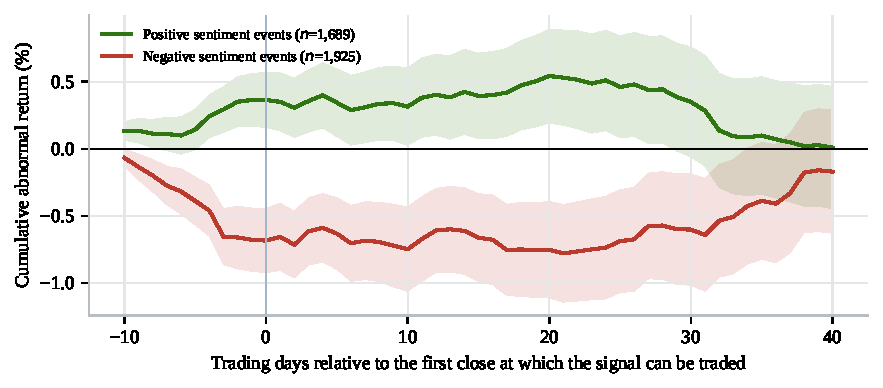
\includegraphics[width=\textwidth]{event_study}
\caption{Cumulative abnormal return (relative to the equal-weighted return of the stock's region) around gauge signals, 2015--2025, with 95\% intervals. Day~0 is the first close at which the signal can be traded.}\label{fig:event}\end{figure}
\begin{multicols}{2}

In Fama--MacBeth regressions (Table~\ref{tab:fm}), a one-standard-deviation higher firm gauge predicts a \FMCtrlFirm{} basis points higher relative return the next week after price controls ($t=\FMCtrlFirmT$), \FMUSFirm{} basis points in the United States ($t=\FMUSFirmT$) and \FMEUFirm{} in the euro area ($t=\FMEUFirmT$). Sector sentiment is insignificant. H1b is supported in direction only for firm sentiment. Over horizons of one to eight weeks the gauge's rank IC is near zero, with its highest value, \DecaySentimentFour{} ($t=\DecaySentimentFourT$), four weeks ahead (Figure~\ref{fig:decay}).
\end{multicols}
\begin{figure}[H]\centering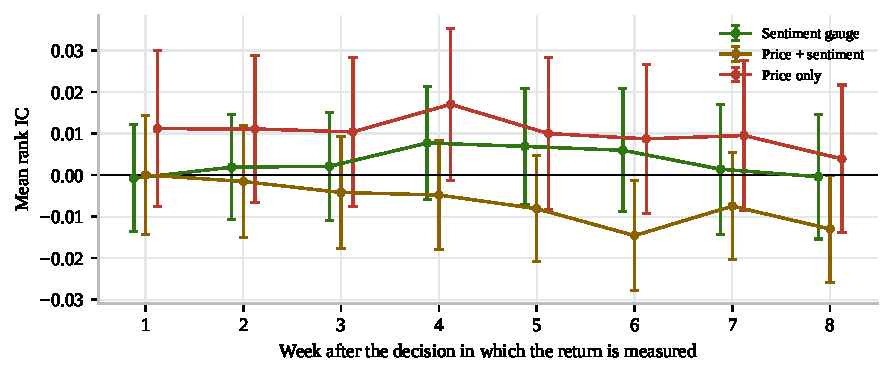
\includegraphics[width=0.85\textwidth]{decay}
\caption{Mean rank IC of each signal for returns one to eight weeks after the decision, with 95\% intervals.}\label{fig:decay}\end{figure}
\begin{table}[H]\centering\footnotesize\begin{tabular}{lcccc}
\toprule
Regressor & Sentiment only & With price controls & U.S. & Euro area \\
\midrule
Firm sentiment gauge & +1.1 (0.97) & +1.3 (1.19) & +2.2 (1.61) & -0.9 (-0.45) \\
Sector sentiment gauge & -1.9 (-0.79) & -0.8 (-0.41) & -1.1 (-0.51) & -0.9 (-0.37) \\
Momentum 12-1 &  & +1.5 (0.55) & +2.5 (0.83) & +2.3 (0.72) \\
Reversal (1 month) &  & +4.9 (1.59) & +5.6 (1.47) & +3.5 (1.24) \\
Volatility (60 days) &  & -3.4 (-0.99) & -2.5 (-0.69) & -2.4 (-0.67) \\
Dollar volume &  & +3.3 (1.22) & +3.5 (1.63) & -3.9 (-1.94) \\
Beta (52 weeks) &  & +7.5 (1.49) & +4.7 (0.87) & +7.2 (1.58) \\
Mean $R^2$ & 0.036 & 0.242 & 0.271 & 0.326 \\
\bottomrule
\end{tabular}

\caption{Fama--MacBeth regressions of next-week relative returns on standardised predictors, 2015--2025. Coefficients in basis points per standard deviation, Newey--West $t$-statistics in parentheses.}\label{tab:fm}\end{table}
\begin{multicols}{2}

\subsection{Sentiment as confirmation of the price forecast (RQ2)}
In the test period the factor composite kept a small positive IC, \ICPrice{} ($t=\ICPriceT$), while the corrected forecast fell to \ICCombined{} ($t=\ICCombinedT$) and the gauge itself had an IC of \ICSentiment{} ($t=\ICSentimentT$). Table~\ref{tab:decisions} shows the hit rates behind this result. The price signal and the sentiment gauge were each right about half of the time, whether they agreed or disagreed. When the correction moved a stock to the other side of the average (\DecChangedShare{} of cases), the original price decision would have been right more often than the new one (\DecChangedPrice{} against \DecChangedComb{}).
\end{multicols}
\begin{table}[H]\centering\footnotesize
\begin{tabular}{lccc}\toprule
\multicolumn{4}{l}{\emph{A. Did each signal pick the right side of the average?}}\\
Situation & Share of cases & Price signal right & Sentiment right\\\midrule
Price and sentiment agree & \DecAgreeShare & \DecAgreePrice & \DecAgreeSent\\
Price and sentiment disagree & \DecDisagreeShare & \DecDisagreePrice & \DecDisagreeSent\\
Sentiment neutral & \DecNeutralShare & \DecNeutralPrice & \DecNeutralSent\\
All cases & \DecAllShare & \DecAllPrice & \DecAllSent\\\midrule
\multicolumn{4}{l}{\emph{B. Decisions changed by the sentiment correction}}\\
 & Share of cases & Original price decision right & Corrected decision right\\\midrule
Correction moved the stock to the other side & \DecChangedShare & \DecChangedPrice & \DecChangedComb\\\bottomrule
\end{tabular}
\caption{Who was right? One case is one stock in one week, 2015--2025. A signal is right when the stock it favours (penalises) does better (worse) than the average stock the next week; a coin flip is right 50\% of the time. Sentiment agrees or disagrees when its gauge is at least 0.5 s.d. on the same or the opposite side of the price signal; cases with a gauge of exactly zero are left out of ``Sentiment right''.}\label{tab:decisions}\end{table}
\begin{multicols}{2}

The portfolio results are better than the forecast results (Table~\ref{tab:performance}). The price + sentiment portfolio earned \CombinedCAGR{} a year with a Sharpe ratio of \CombinedSharpe{} and a maximum drawdown of \CombinedDD{}, against \PriceCAGR{}, \PriceSharpe{} and \PriceDD{} for price only; the difference, \BootCombinedPriceCAGR{} percentage points a year, has a 95\% interval of [\BootCombinedPriceCAGRLow, \BootCombinedPriceCAGRHigh] (Table~\ref{tab:uncertainty}). Figure~\ref{fig:mechanism} shows where the difference arises. As a simple average, the gain of \NetCombinedPrice{} percentage points a year splits into \GrossCombinedPrice{} before costs and \SavingCombinedPrice{} from lower costs. The before-cost gain came equally from the price portfolio's buy decisions (stocks it overweighted; \SideBuyGain{} percentage points a year, $t=\SideBuyGainT$) and sell decisions (stocks it underweighted; \SideSellGain, $t=\SideSellGainT$). When sentiment enlarged a buy or a sell, the stock moved the intended way in \SideBuyLargerRight{} and \SideSellLargerRight{} of cases. H2a and H2b are supported in direction but not statistically, and H2c in direction only: stocks moved \DecAgreeRet{} basis points a week in the price signal's direction when sentiment agreed and \DecDisagreeRet{} when it disagreed (both insignificant).
\end{multicols}
\begin{figure}[H]\centering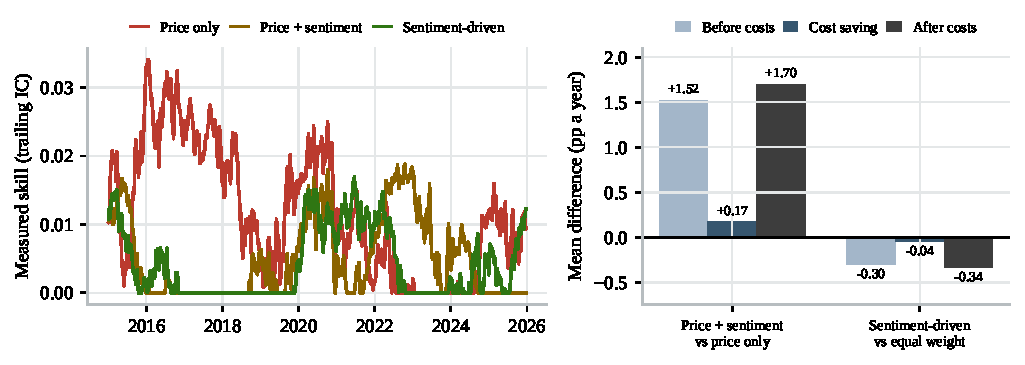
\includegraphics[width=\textwidth]{allocation_mechanism}
\caption{Left: measured skill (trailing three-year rank IC, floored at zero) that scales each signal's views. Right: mean annual return difference before costs, from lower costs and after costs (arithmetic, percentage points).}\label{fig:mechanism}\end{figure}
\begin{multicols}{2}

\subsection{Sentiment as the driver of the allocation (RQ3)}
Driven by sentiment alone, the portfolio held about \SentimentHoldings{} stocks with views on \SentimentViews{} of them in an average week; in \ZeroSkillSentiment{} of the weeks the gauge's trailing IC was zero and the optimiser moved towards equal weighting. The portfolio earned \SentimentCAGR{} a year, slightly less than equal weighting (\EWCAGR), but with a Sharpe ratio of \SentimentSharpe{}, against \EWSharpe{} for equal weighting, \MinVarSharpe{} for minimum variance and \IndexSharpe{} for MSCI World (Figure~\ref{fig:wealth}; drawdowns and annual returns in Appendix~\ref{app:annual}). Its maximum drawdown, \SentimentDD{}, was smaller than that of equal weighting (\EWDD{}) and the index (\IndexDD{}). All differences have bootstrap intervals that include zero (Table~\ref{tab:uncertainty}). H3 is supported in direction only.
\end{multicols}
\begin{table}[H]\centering\footnotesize\setlength{\tabcolsep}{4pt}\begin{tabular}{lrrrrrrrrr}
\toprule
Strategy & CAGR & Vol. & Sharpe & Sortino & Max DD & Turnover & Costs & $\alpha$ ($t$) & $\beta$ \\
\midrule
Sentiment-driven & 11.90 & 16.77 & 0.64 & 0.89 & -31.6 & 1.6 & 0.17 & +1.59 (+0.67) & 0.91 \\
Price + sentiment & 12.20 & 16.86 & 0.65 & 0.93 & -30.4 & 3.5 & 0.36 & +1.62 (+0.81) & 0.93 \\
Price only & 10.28 & 16.99 & 0.54 & 0.76 & -34.4 & 5.2 & 0.54 & -0.11 (-0.05) & 0.94 \\
Minimum variance & 9.41 & 13.05 & 0.60 & 0.81 & -28.2 & 0.5 & 0.05 & +1.15 (+0.55) & 0.67 \\
Equal weight & 12.15 & 17.46 & 0.63 & 0.90 & -36.7 & 1.2 & 0.13 & +1.30 (+0.65) & 0.97 \\
MSCI World (URTH) & 11.18 & 16.59 & 0.60 & 0.85 & -32.7 & -- & -- & -- & -- \\
\bottomrule
\end{tabular}

\caption{Net performance, January 2015 to December 2025 (\Weeks{} weeks), 10 bp per trade. CAGR, volatility, costs and alpha in \% a year; turnover is the average weekly one-way turnover in \%; alpha and beta against MSCI World with Newey--West $t$-statistics.}\label{tab:performance}\end{table}
\begin{table}[H]\centering\footnotesize\setlength{\tabcolsep}{4pt}\begin{tabular}{lcccc}
\toprule
Comparison (A vs B) & Return (pp a year) & Sharpe ratio & Drawdown (pp) & Significant? \\
\midrule
Price + sentiment vs price only & +1.92 (-1.47 to +5.00) & +0.10 (-0.09 to +0.28) & +4.0 (-5.5 to +9.5) & No \\
Sentiment-driven vs equal weight & -0.25 (-3.23 to +2.72) & +0.01 (-0.15 to +0.14) & +5.1 (-3.9 to +9.1) & No \\
Sentiment-driven vs minimum variance & +2.49 (-3.09 to +8.62) & +0.03 (-0.32 to +0.34) & -3.3 (-13.9 to +2.7) & No \\
Sentiment-driven vs MSCI World & +0.72 (-4.01 to +5.76) & +0.03 (-0.24 to +0.29) & +1.1 (-6.2 to +10.4) & No \\
Price + sentiment vs equal weight & +0.06 (-2.41 to +2.56) & +0.02 (-0.12 to +0.14) & +6.3 (-4.0 to +10.7) & No \\
Price only vs equal weight & -1.86 (-5.20 to +1.43) & -0.09 (-0.26 to +0.08) & +2.2 (-5.0 to +6.8) & No \\
\bottomrule
\end{tabular}

\caption{Are the differences real? Each cell shows strategy A minus strategy B (for drawdown, how much smaller A's drawdown was) with its 95\% confidence interval in brackets (paired block bootstrap, 13-week blocks, 2,000 draws). A difference is significant only if its interval excludes zero.}\label{tab:uncertainty}\end{table}
\begin{figure}[H]\centering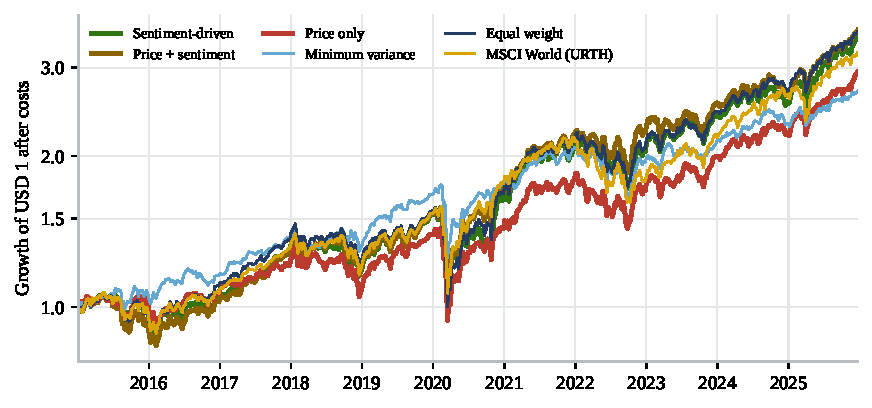
\includegraphics[width=\textwidth]{wealth}
\caption{Growth of USD~1 after costs, 2015--2025 (log scale).}\label{fig:wealth}\end{figure}
\begin{multicols}{2}
